\section{Tree Types \& Traversals}

\subsection{Binary Trees: 2 Children}

\noindent
First we'll define a basic binary tree and then all its extensions.
\begin{Def}[Binary Tree]

    A \textbf{binary tree} is a tree where each parent node has at most two children.
\end{Def}

\begin{figure}[h]
    \begin{center}
    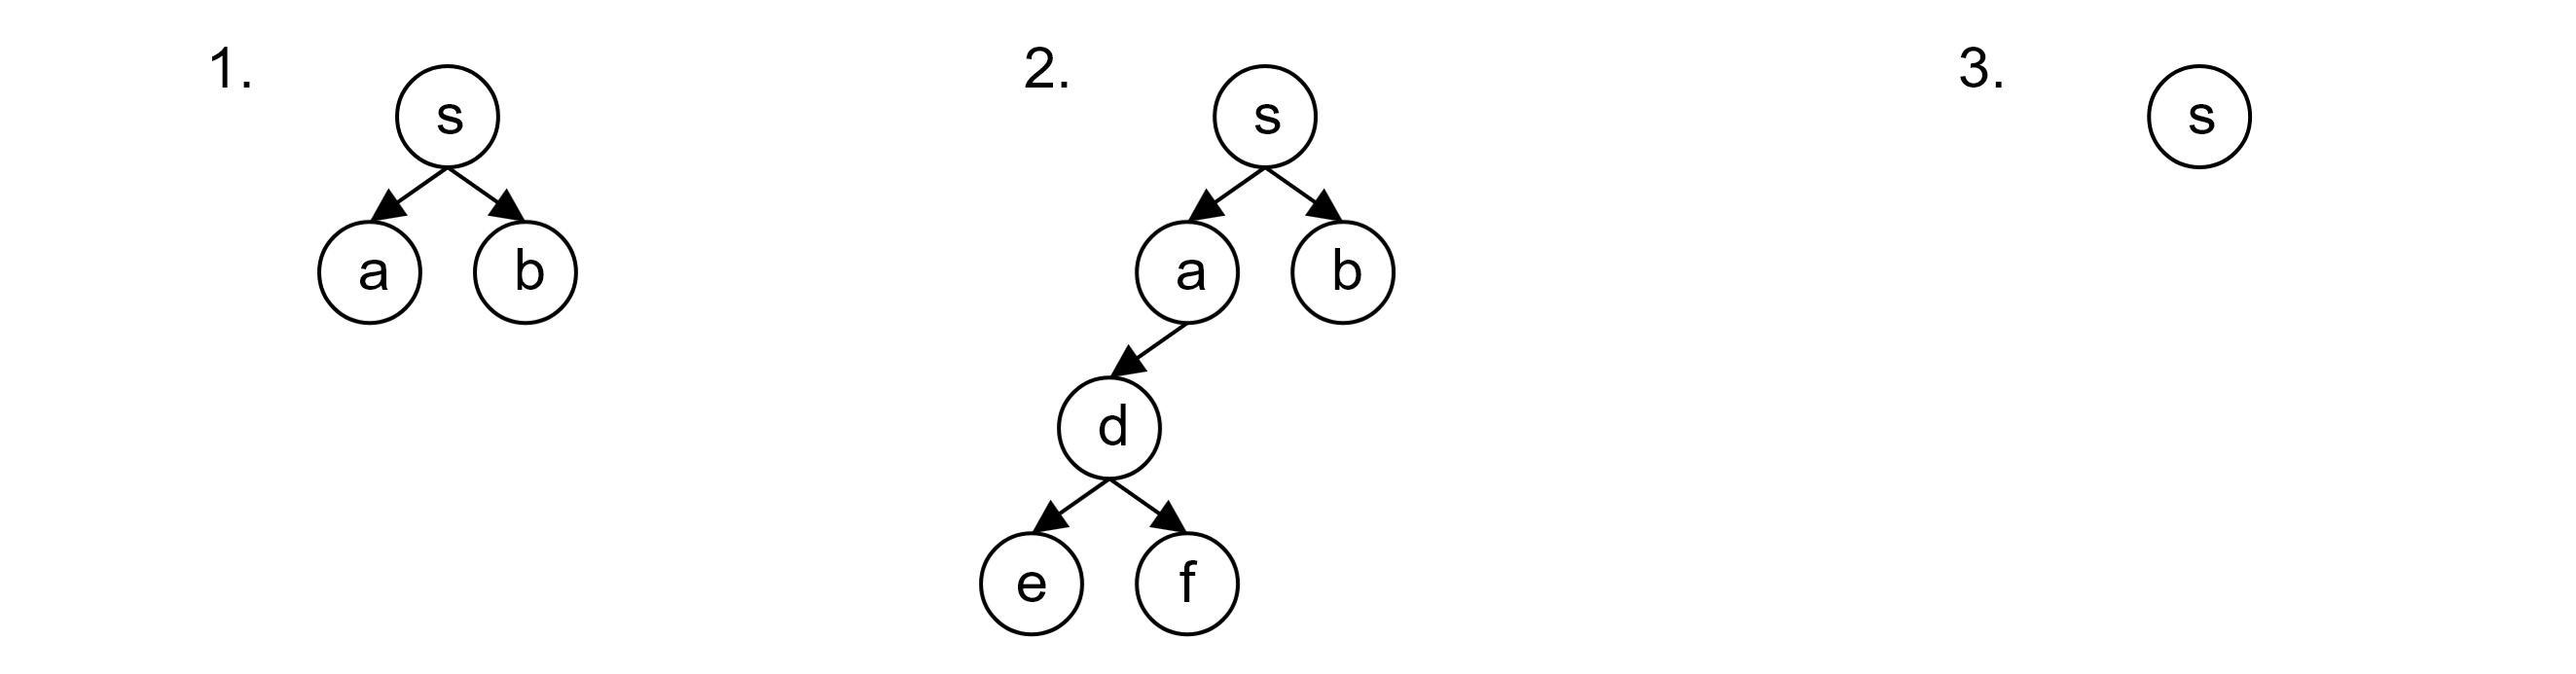
\includegraphics[width=\textwidth]{./Sections/graphs/binary_tree.png}
    \end{center}
     \caption{These are three examples of binary trees, including a single node (3).}\label{fig:binary_tree}
  \end{figure}

\noindent
To simply do a binary tree traversal, we may employ the following methods:
\begin{Func}[DFS Binary Tree Traversal - \texttt{DFS($T$)}]
    Depth-First Search on binary tree $T$ (recursive).
    
    \vspace{.5em}
    \noindent
    \textbf{Input:} Binary tree $T$.\\
    \textbf{Output:} Nodes in pre-order, in-order, and post-order.
    
    \begin{algorithm}[H]
        \SetAlgoLined
        \SetKwProg{Fn}{Function}{:}{}
        \Fn{\texttt{DFS($T$)}}{
            \If{$T$ is not empty}{
                Visit node $T$\;
                \texttt{DFS($T.left$)}\;
                \texttt{DFS($T.right$)}\;
            }
        }
    \end{algorithm}
    \noindent
    \rule{\textwidth}{0.4pt}
    \textbf{Time Complexity:} Given n nodes, and a force of a tree format, we have $n-1$ edges. Therefore with $m$ edges, $n+m = n+(n-1)$, hence $O(n)$ time.\\
    \textbf{Space Complexity:} again, we have $O(n)$ space for the stack.
\end{Func}

\noindent
$\mathbf{\rightarrow}$ \textbf{\underline{BFS has the same complexities} as per the same reasoning as the above function.}\\

\newpage
\noindent
The order in the above function is called \textbf{pre-order traversal};

\begin{Def}[Order Traversals]

    The order of traversal refers to the order in which nodes are visited/processed:
    \begin{itemize}
        \item \textbf{Pre-order:} Visit the node, then left, then right.
        \item \textbf{In-order:} Visit left, then the node, then right.
        \item \textbf{Post-order:} Visit left, then right, then the node.
    \end{itemize}
    In particular, \underline{\textbf{in-order traversal} is simply a run of \textbf{BFS}} as it processes the tree level by level starting 
    from the root.
\end{Def}

\noindent
Below is an example of all three:

\begin{Example}[Binary Tree Traversals (Part 1)]

    \begin{lstlisting}[language=Python, numbers=none]
    # Pre-order Traversal
    def PreOrder(T):
        if T is not None:
            visit(T)
            PreOrder(T.left)
            PreOrder(T.right)

    # In-order Traversal
    def InOrder(T):
        if T is not None:
            InOrder(T.left)
            visit(T)
            InOrder(T.right)

    # Post-order Traversal
    def PostOrder(T):
        if T is not None:
            PostOrder(T.left)
            PostOrder(T.right)
            visit(T)

    # Level-order Traversal
    def LevelOrder(T):
        BFS(T)
    \end{lstlisting}
\end{Example}

\newpage

\noindent
Now to show how this actually looks:
\begin{figure}[h]


    \hspace {-10em} 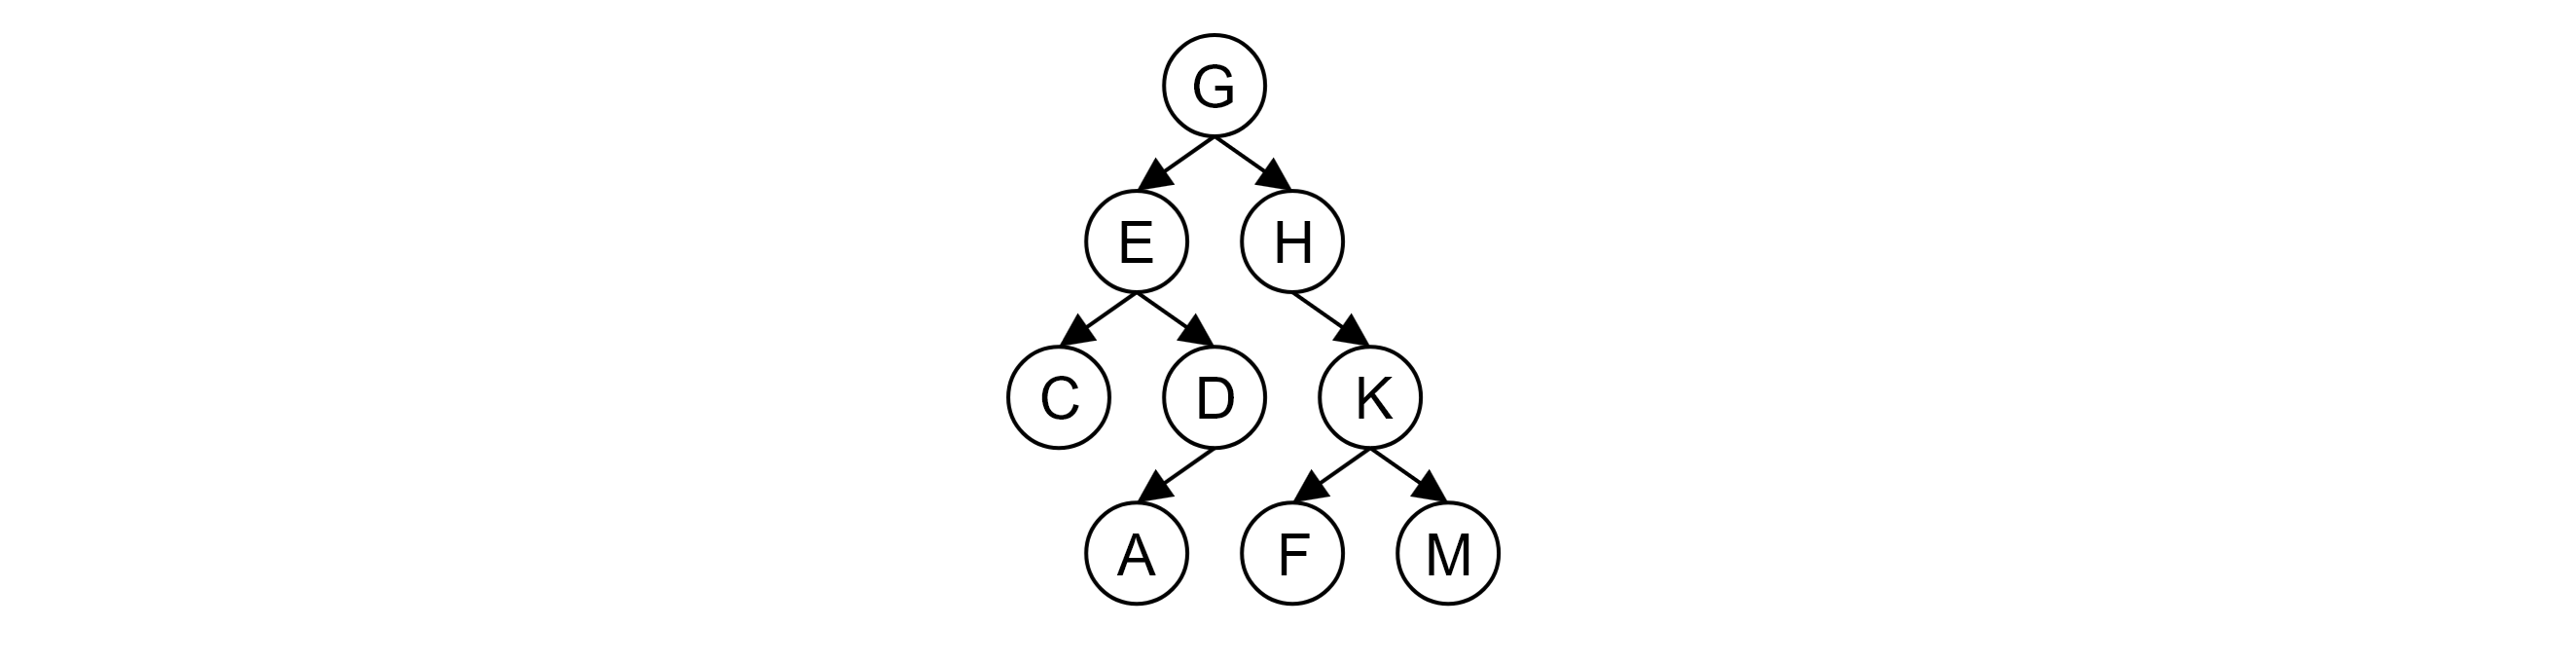
\includegraphics[width=1.5\textwidth]{./Sections/graphs/binary_tree_traversals.png}
  
     \caption{%
        The above binary tree has the following traversals:\\[1em]
           $\bullet$\quad  \textbf{Pre-order:}  \hspace{.5em} G, E, C, D, A, H, K, F, M\\
           $\bullet$\quad  \textbf{In-order:}   \hspace{1.2em} C, E, A, D, G, H, F, K, M\\
           $\bullet$\quad  \textbf{Post-order:} \hspace{.05em} C, A, D, E, F, M, K, H, G\\
           $\bullet$\quad \textbf{Level-order:} G, E, H, C, D, K, A, F, M\\[1em]
         Notably, if there is no left or right child to explore for that particular traversal order, that node then and there is processed.
     For example, in in-order traversal, since $C$ has no left child, it is processed first. The same goes for Post-order, where $D$ has no right child, so it is processed.
     }\label{fig:binary_tree_traversals}
  \end{figure}

\begin{Def}[Types of Binary Trees]

    There are several types of binary trees, each with its own properties:
    \begin{itemize}
        \item \textbf{Full Binary Tree:} Every node has either 0 or 2 children.
        \item \textbf{Complete Binary Tree:} All levels are fully filled except possibly the last level, which is filled from left to right.
        \item \textbf{Perfect Binary Tree:} All interior nodes have two children and all leaves are at the same level.
        \item \textbf{Balanced Binary Tree:} The height of the left and right subtrees of every node differ by at most one.
    \end{itemize}
    \noindent
    \textbf{Note:} A full binary tree is not necessarily complete, and a complete binary tree is not necessarily full.
\end{Def}

\newpage

\noindent
Observe the following examples of binary trees:
\begin{figure}[h]
    \begin{center}
    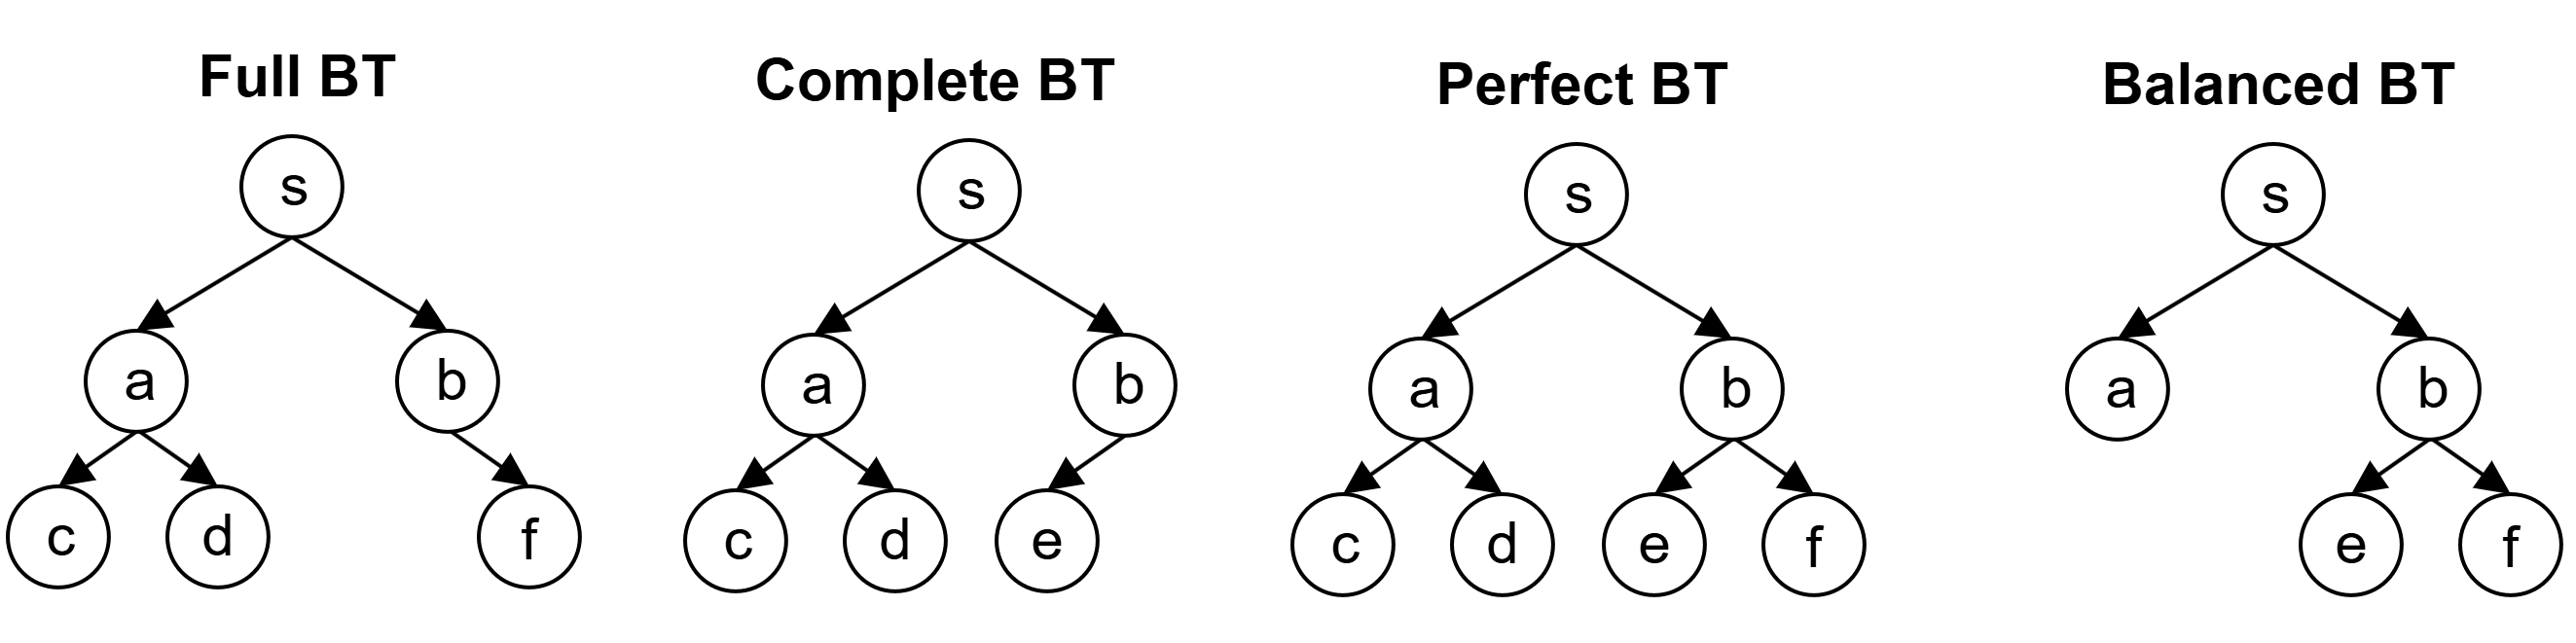
\includegraphics[width=\textwidth]{./Sections/graphs/search/binary_tree_types.png}
    \end{center}
     \caption{These are examples of different types of binary trees (BT).}\label{fig:binary_tree_types}
  \end{figure}


\subsection{Binary Search Tree}
\noindent
A binary search tree is a stricter form of a binary tree, which gives us an efficient search algorithm.
\begin{Def}[Binary Search Tree (BST) -- Overview]

    \label{def:binary_search_tree}

    A \textbf{binary search tree} is a binary tree where:
    
    \begin{center}
        left child $<$ parent node $\leq$ right child
    \end{center}
    \noindent
    \textbf{Note:} A Binary Tree \underline{\textbf{is not}} a Binary Search Tree, unless it satisfies the above conditions.
\end{Def}

\begin{figure}[h]
    \begin{center}
    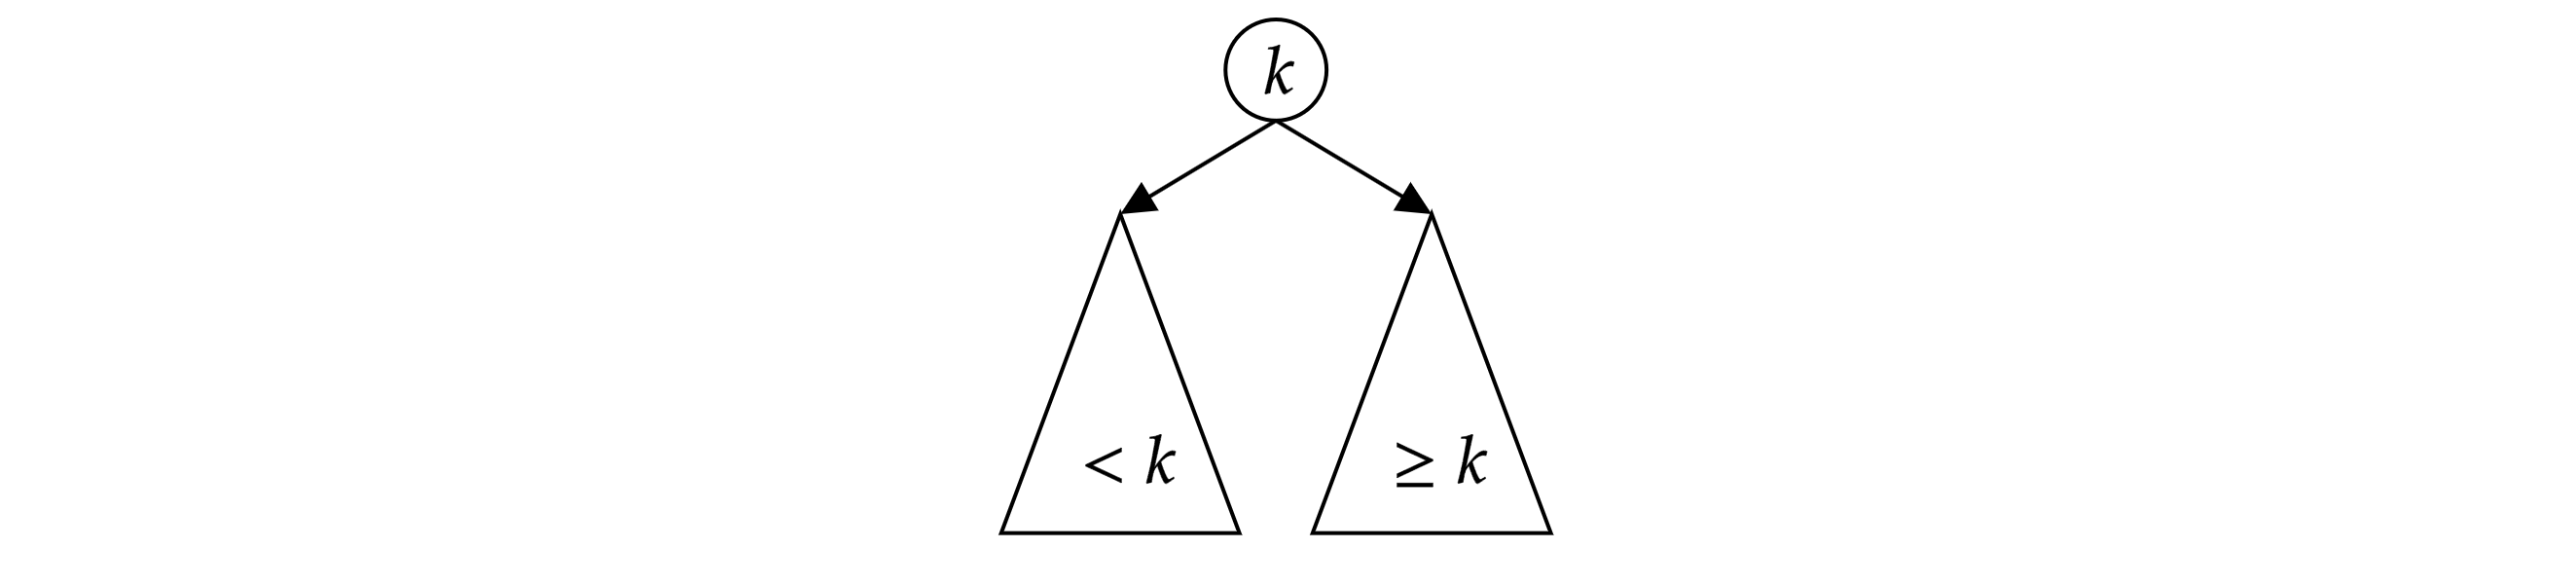
\includegraphics[width=\textwidth]{./Sections/graphs/search/bst.png}
    \end{center}
     \caption{Visual Representation of Definition (\ref{def:binary_search_tree}), where $k$ is 
     the parent node with its respective left (less than) and right (greater than or equal to) nodes.}\label{fig:binary_search_tree}
  \end{figure}

\noindent
The next few pages we discuss \textbf{Searching, Insertion, and Deletion} in a binary search tree.
  
\newpage
\begin{Func}[Binary Search Tree (BST) -- Searching]

    Given a BST root node $T$ and a desired value $v$, we can search for $v$ in $T$ as follows:
  \newpage 
    \vspace{.5em}
    \noindent
    \textbf{Input:} BST root node $T$, value $v$.\\
    \textbf{Output:} Node containing $v$ or null if not found.
    
    \begin{algorithm}[H]
        \SetAlgoLined
        \SetKwProg{Fn}{Function}{:}{}
        \Fn{\texttt{Search($T, v$)}}{
            \While{$T$ is not null}{
                \If{$T.value = v$}{
                    \KwRet{$T$}\;
                }
                \If{$v < T.value$}{
                    $T \gets T.left$\;
                }
                \Else{
                    $T \gets T.right$\;
                }
            }
            \KwRet{null}\;
        }
    \end{algorithm}
    \noindent
    \rule{\textwidth}{0.4pt}
    \textbf{Time Complexity:} $O(h)$ where $h$ is the height of the tree. In a balanced BST, this is $O(\log n)$, but in the worst case (unbalanced), it can be $O(n)$.
\end{Func}

\begin{figure}[ht!]
    \begin{center}
    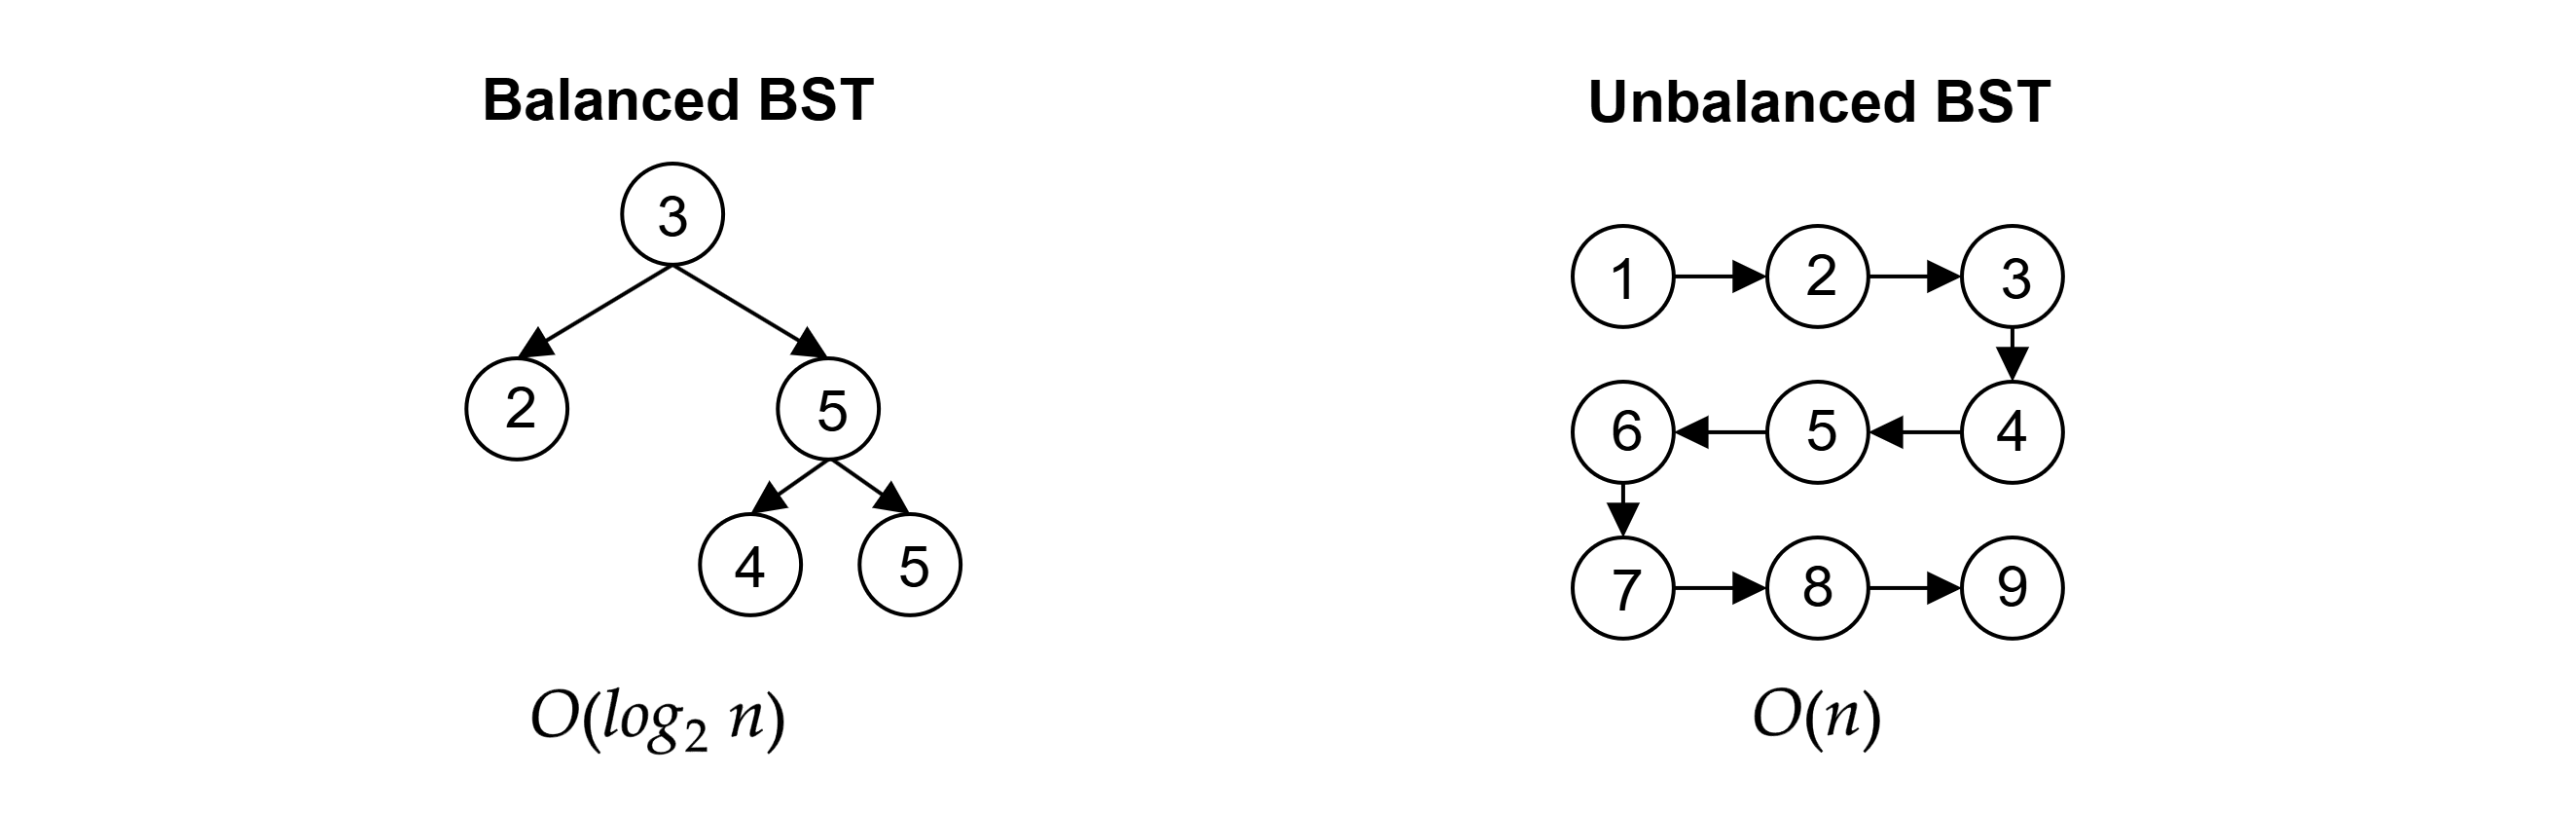
\includegraphics[width=\textwidth]{./Sections/graphs/search/bst_search.png}
    \end{center}
     \caption{Searching for a value in a binary search tree. The worst case is a noodle (all right nodes), forcing $n$ traversals, i.e., the height (within a constant). One could imagine these nodes as complex objects, where the value $v$ is a key, and the node itself contains more data.}\label{fig:bst_search}
  \end{figure}

\begin{theo}[Property of Binary Search Trees]

    \label{theo:bst_property}

    In a binary search tree, for any node $N$:
    \begin{itemize}
        \item All values in the left subtree of $N$ are less than the value of $N$.
        \item All values in the right subtree of $N$ are greater than or equal to the value of $N$.
    \end{itemize}
\end{theo}

\newpage 
\noindent
Insertion is the same an searching, except we insert upon reaching a null node.
\begin{Func}[Binary Search Tree (BST) -- Insertion]

    Given a BST root node $T$ and a value $v$, we can insert $v$ into $T$ as follows:
    
    \vspace{.5em}
    \noindent
    \textbf{Input:} BST root node $T$, value $v$.\\
    \textbf{Output:} Updated binary search tree with $v$ inserted.
    
    \begin{algorithm}[H]
        \SetAlgoLined
        \SetKwProg{Fn}{Function}{:}{}
        \Fn{\texttt{Insert($T, v$)}}{
            $parent \gets$ null; $current \gets T$\;
            \While{$current$ is not null}{
                $parent \gets current$\;
                \If{$v < current.value$}{
                    $current \gets current.left$\;
                }
                \Else{
                    $current \gets current.right$\;
                }
            }
            \vspace{1em}
            \tcp{After the while loop terminates}
            \If{$parent$ is null}{
                \KwRet{$v$} \tcp*[l]{Tree was empty, $v$ becomes root}
            }
            \If{$v < parent.value$}{
                $parent.left \gets v$\;
            }
            \Else{
                $parent.right \gets v$\;
            }
            \KwRet{$T$}\;
        }
    \end{algorithm}
    \noindent
    \rule{\textwidth}{0.4pt}
    \textbf{Time Complexity:} $O(h)$ where $h$ is the height of the tree. In a balanced BST, this is $O(\log n)$, but in the worst case (unbalanced), it can be $O(n)$.\\
\end{Func}

\noindent
Deletion is a bit more complex, as we have to consider removing intermediate nodes:

\begin{theo}[Binary Search Tree (BST) -- Deletion]

    When deleting a node from a binary search tree, we must consider three cases:
    \begin{itemize}
        \item \textbf{$v$ has no children:} Remove the parent's reference to $v$.
        \item \textbf{$v$ has one child:} Replace the parent's reference to $v$'s child.
        \item \textbf{$v$ has two children:} Replace the parent's reference to $v$ with either:
            \begin{itemize}
                \item The \textbf{L}argest value in $v$'s \textbf{L}eft subtree (in-order predecessor).
                \item The \textbf{R}unt (smallest) value in $v$'s \textbf{R}ight subtree (in-order successor).
            \end{itemize}
    \end{itemize}

    \noindent
    This ensures that the binary search tree properties are maintained after deletion.
\end{theo}

\newpage
\begin{Func}[Binary Search Tree (BST) -- Deletion]

    Given a BST root node $T$ and a value $v$, we can delete $v$ from $T$ as follows:
    
    \vspace{.5em}
    \noindent
    \textbf{Input:} BST root node $T$, value $v$.\\
    \textbf{Output:} Updated binary search tree with $v$ deleted.
    
    \begin{algorithm}[H]
        \SetAlgoLined
        \SetKwProg{Fn}{Function}{:}{}
        \Fn{\texttt{Delete($T, v$)}}{
            $parent \gets$ null; $current \gets T$\;
            \While{$current$ is not null \textbf{and} $current.value \neq v$}{
                $parent \gets current$\;
                \If{$v < current.value$}{
                    $current \gets current.left$\;
                }
                \Else{
                    $current \gets current.right$\;
                }
            }
            \If{$current$ is null}{
                \KwRet{$T$} \tcp*[l]{Value not found}
            }
            \tcp{Case 1: Node has at most one child}
            \If{$current.left$ is null \textbf{or} $current.right$ is null}{
                \If{$current.left$ is not null}{
                    $child \gets current.left$\;
                }
                \Else{
                    $child \gets current.right$\;
                }
                \If{$parent$ is null}{
                    \KwRet{$child$} \tcp*[l]{Deleted root}
                }
                \If{$parent.left = current$}{
                    $parent.left \gets child$\;
                }
                \Else{
                    $parent.right \gets child$\;
                }
                \KwRet{$T$}\;
            }
            \tcp{Case 2: Node has two children}
            $succParent \gets current$\;
            $succ \gets current.right$ \tcp*[l]{Runt of Right subtree}
            \While{$succ.left$ is not null}{
                $succParent \gets succ$\;
                $succ \gets succ.left$\;
            }
            $current.value \gets succ.value$\;
            \If{$succParent.left = succ$}{
                $succParent.left \gets succ.right$\;
            }
            \Else{
                $succParent.right \gets succ.right$\;
            }
            \KwRet{$T$}\;
        }
    \end{algorithm}
    \noindent
    \rule{\textwidth}{0.4pt}
    \textbf{Time Complexity:} $O(h)$ where $h$ is the height of the tree. In a balanced BST, this is $O(\log n)$, but in the worst case (unbalanced), it can be $O(n)$.
\end{Func}

\newpage 

\noindent
Consider an example as we build a binary search tree and performing the above operations:
\begin{figure}[h]
    \centering
    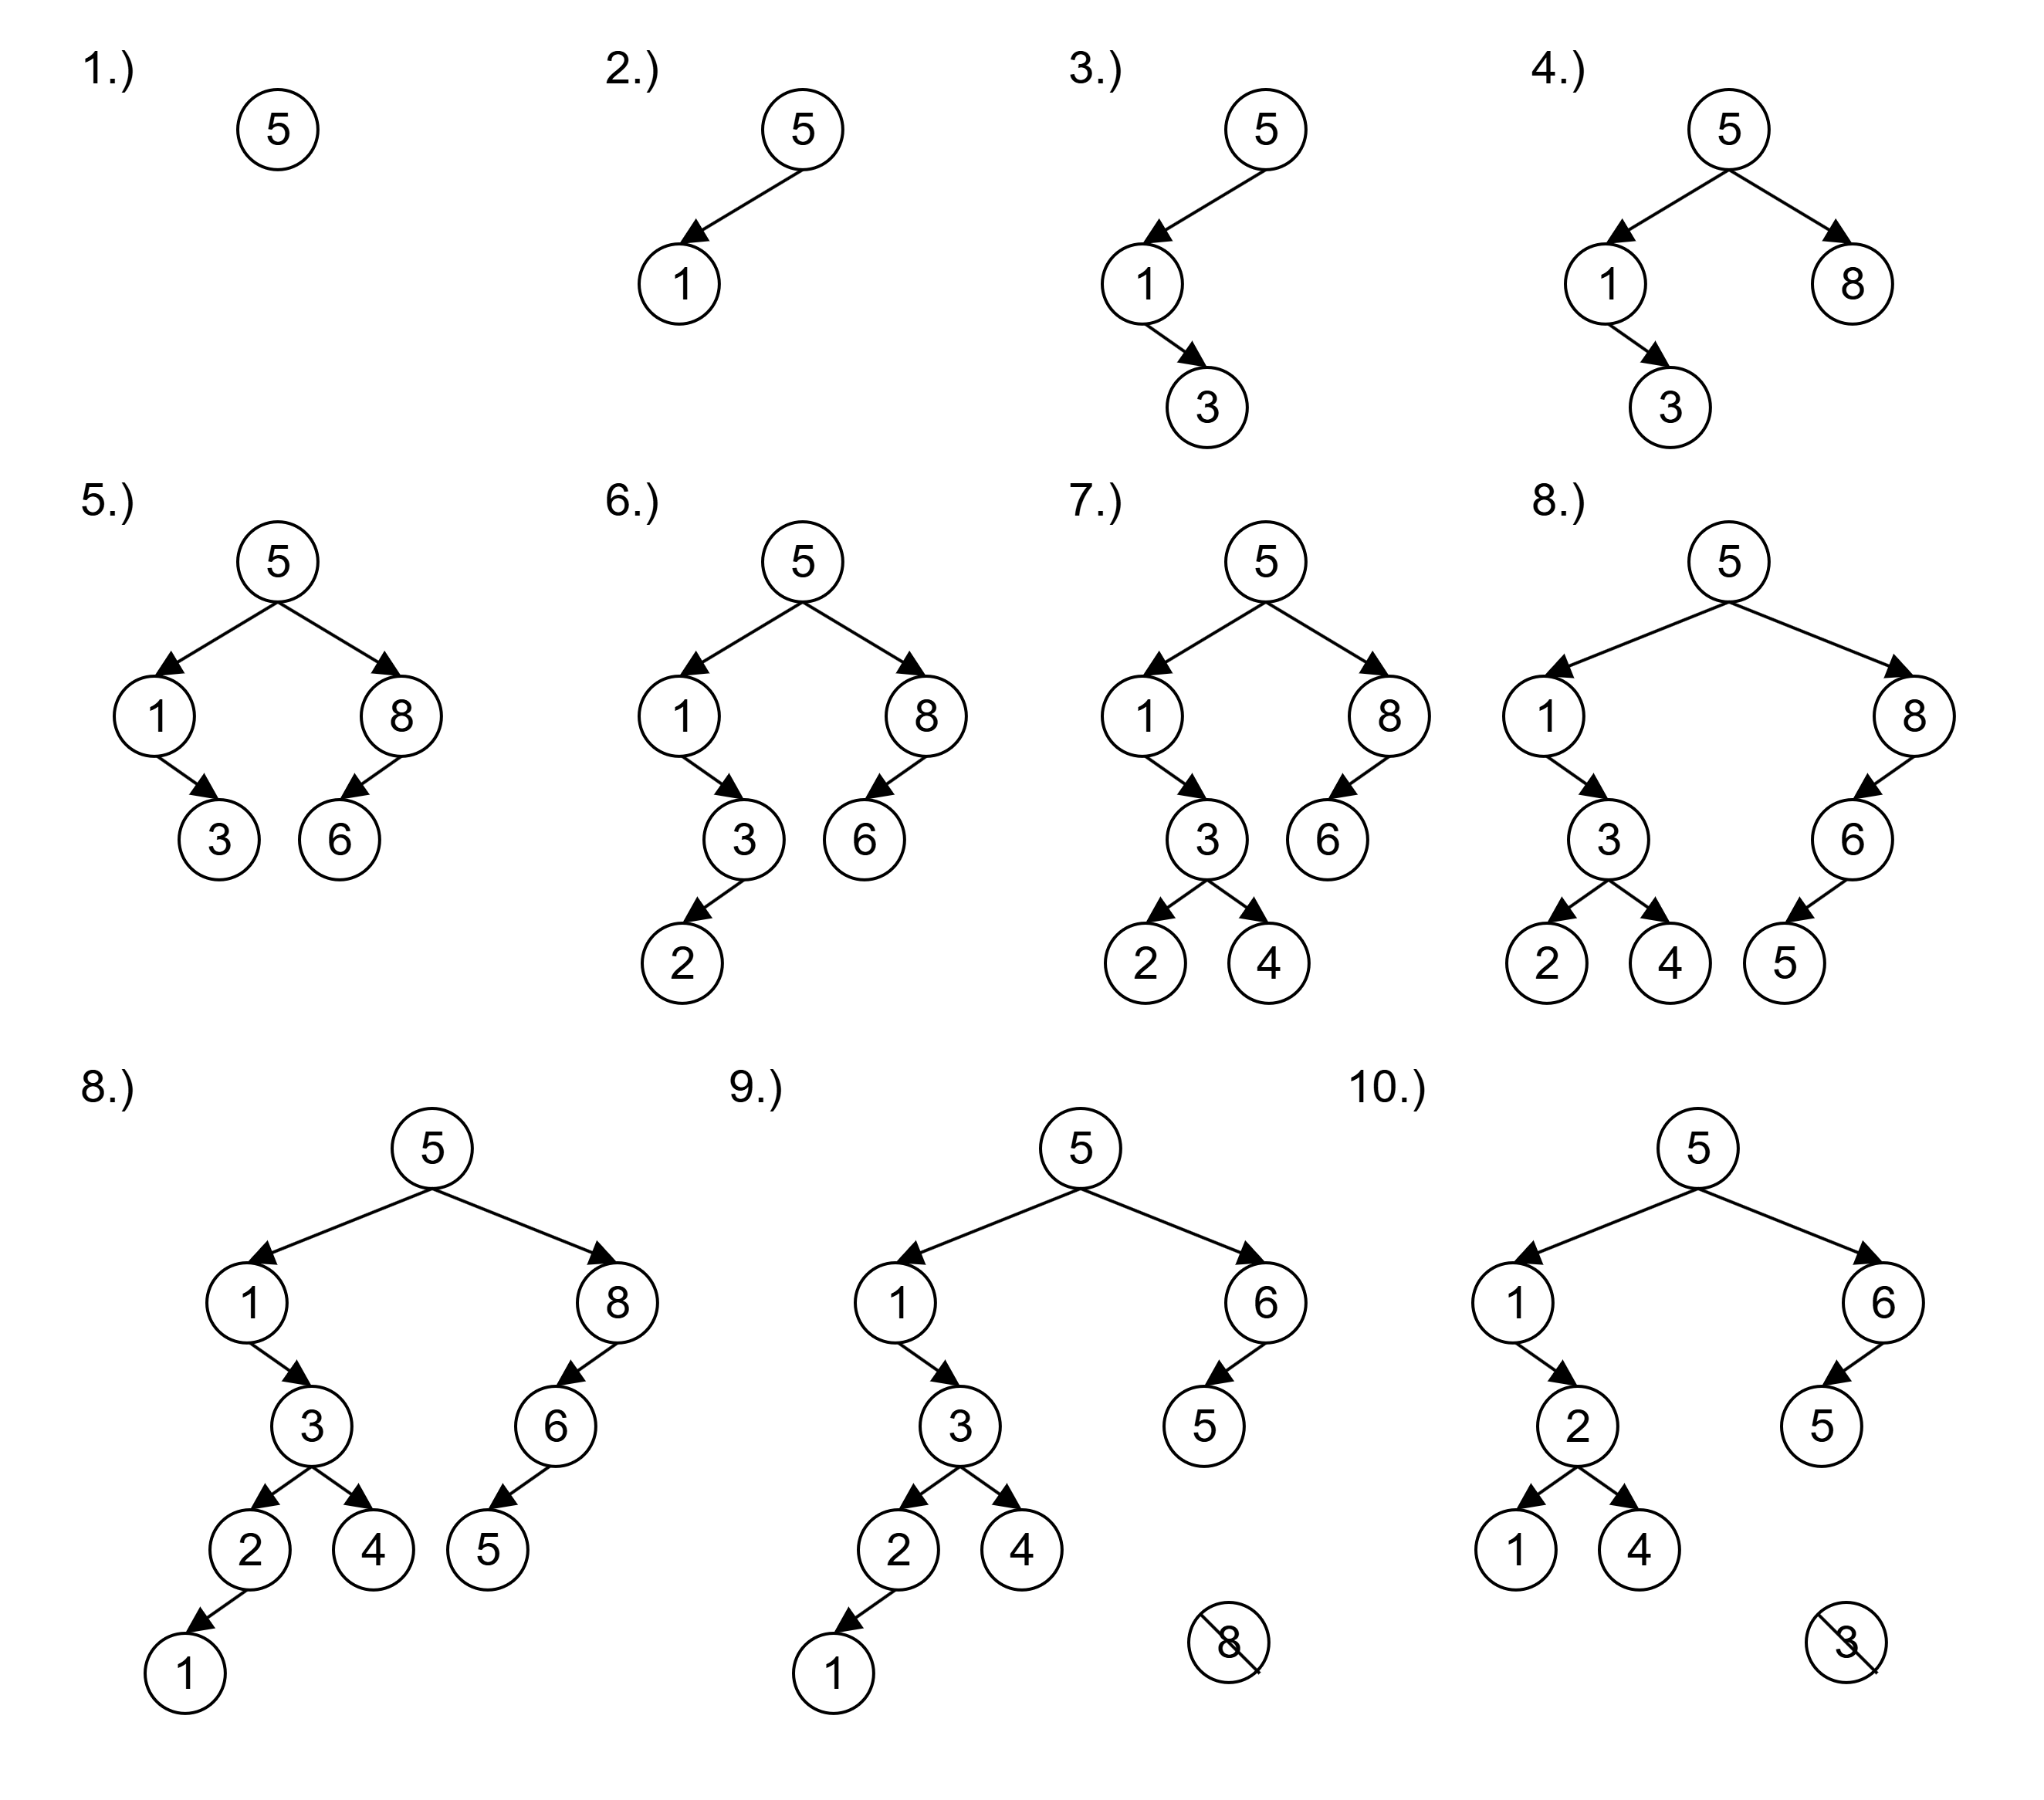
\includegraphics[width=\textwidth]{./Sections/graphs/search/bst_ex.png}
    \caption{%
        \textbf{Note:} We use the Largest Left child (in-order predecessor) to replace the 2-children case. From 
        1--9 we insert values. From 10--11 we delete. In (10) we delete 8 (1-child case), we replace its 
        parent's reference to 8 with its only child 6. In (11) we delete 3 (2-children case), we replace its parent's reference to 3 with the largest left child, which is 2.
        One could imagine the in-order successor (smallest right child) would have 4 instead of 2, with 2 and 1 on its left subtree.}
    \label{fig:bst_operations}
\end{figure}

\newpage 
\subsection{2-3 Trees: 3 Children Search}

\noindent
We can keep extending the binary tree to allow for more children, which allows us to search faster.
\begin{Def}[Ternary \& N-ary Trees]

    A \textbf{ternary tree} is a tree where each parent node has at most three children. An \textbf{n-ary tree} is a tree where each parent node can have up to $n$ children.
\end{Def}

\noindent
The following is a specific arrangement of a ternary tree, akin to binary trees and binary search trees. So 
far we've discussed structures where each node has 1 key, but this changes with 2-3 trees:
\begin{Def}[2-3 Tree -- Overview]

    A \textbf{2-3 tree} is a balanced search tree where a parent may contain 1 or 2 keys:
    \begin{itemize}
        \item \textbf{1 Key (1K):} This parent has 2 children.
        \item \textbf{2 Keys (2K):} This parent has 3 children.
    \end{itemize}
    \noindent
    The 1K node abides by the same rules as a BST:
    \begin{center}
        left child $<$ parent node $\leq$ right child
    \end{center}
    \noindent
    For 2K let us define the left key as $k_1$ and the right key as $k_2$, then the rules are :
    \begin{center}
        left child $<$ $k_1$ $\leq$ middle child $<$ $k_2$ $\leq$ right child
    \end{center}
    \noindent
    \rule{\textwidth}{0.4pt}
    \textbf{Time Complexity:} Searching, inserting, and deleting in a 2-3 tree is $O(\log n)$, where $n$ is the number of keys in the tree.
    The performance gain comes from 3 children possibility: if the tree has only 3 children, it would be 
    $O(\log_3 n)$, which is faster than $O(\log_2 n)$; However, the tree has have a mix of 1K and 2K nodes.
    So that's why in the worst case, we have $O(\log_2 n)$. I.e., $\lfloor{\log_3 n}\rfloor \leq h \leq \lfloor{\log_2 n}\rfloor$, where $h$ is the height of the tree.
\end{Def}
\newpage